\documentclass{standalone}
\usepackage{tikz,tikz-3dplot}

\usetikzlibrary{math}

\begin{document}

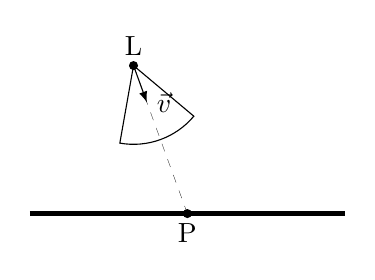
\begin{tikzpicture}
  \tikzmath{
    real \pangle, \lhangle, \startangle, \endangle;
    \pangle=110;
    \lhangle=30;
    \startangle=180+\pangle+\lhangle;
    \endangle=180+\pangle-\lhangle;
  }
  \coordinate (L) at (\pangle:2);
  \coordinate (P) at (0,0);

  \draw[ultra thick] (-2,0) -- (2,0);
  \draw[fill] (L) circle[radius=0.05] node[above] {L};
  \draw[fill] (P) circle[radius=0.05] node[below] {P};
  \draw[-latex] (L) -- ($ (L) ! 0.5cm ! (P) $) node[right] {$\vec{v}$};
  \draw[ultra thin,dashed] (L) -- (P);

  \draw (L) -- ++(\startangle:1) arc[start angle=\startangle,end angle=\endangle,radius=1] -- cycle;
\end{tikzpicture}

\end{document}
